\documentclass[aspectratio=169,fleqn]{beamer}
\PassOptionsToPackage{english}{babel}
\usepackage{standardslides}

\usepackage{svg}

\usepackage{tikz}
\usepackage{pifont}
\usepackage{listings}
\usepackage{colortbl}
\newlength{\listingframemargin}
\setlength{\listingframemargin}{1em}
\newlength{\listingmargin}
\setlength{\listingmargin}{0.08\textwidth}

\definecolor{codeDarkGray}{gray}{0.2}
\definecolor{codeGray}{gray}{0.4}
\definecolor{codeLightGray}{rgb}{0.94,0.94,0.91}
\definecolor{codeBorder}{rgb}{0.34,0.24,0.21}
\definecolor{MidnightBlue}{rgb}{0.1, 0.1, 0.8}

\lstdefinestyle{standard}{%
  belowcaptionskip=0.5\baselineskip,
  breaklines=true,
  frameround=tttt,
  % frame=false,
  xleftmargin=0em,
  xrightmargin=0em,
  showstringspaces=false,
  showtabs=false,
  % tab=\smash{\rule[-.2\baselineskip]{.4pt}{\baselineskip}\kern.5em},
  basicstyle= \fontfamily{pcr}\selectfont\tiny\bfseries,
  keywordstyle= \bfseries\color{MidnightBlue}, %\color{codeDarkGray},
  commentstyle= \itshape\color{codeGray},
  identifierstyle=\color{codeDarkGray},
  stringstyle=\color{BurntOrange}, %\color{codeDarkGray},
  numberstyle=\tiny\ttfamily,
  % numbers=left,
  numbersep = 1em,
  % stepnumber = 1,
  % captionpos=t,
  tabsize=2,
  % backgroundcolor=\color{codebLightGray},
  rulecolor=\color{codeBorder},
  framexleftmargin=\listingframemargin,
  framexrightmargin=\listingframemargin
}

\newcommand{\inputCodeBlock}[1]{%
  % \begin{mybox}
    \begin{center}
      % \begin{minipage}[c]{0.7\textwidth}
        \lstinputlisting[%
          style = standard,
          language = c++,
          morekeywords={constexpr,noexcept,decltype,size_t,uint32_t,uint64_t,__m256i,__m256,__m256d,__m128i,__m128,__m128d}
        ]{#1}
      % \end{minipage}
    \end{center}
  % \end{mybox}
}

\def\UrlBigBreaks{\do\/\do-\do:}

\setbeamertemplate{background}{
  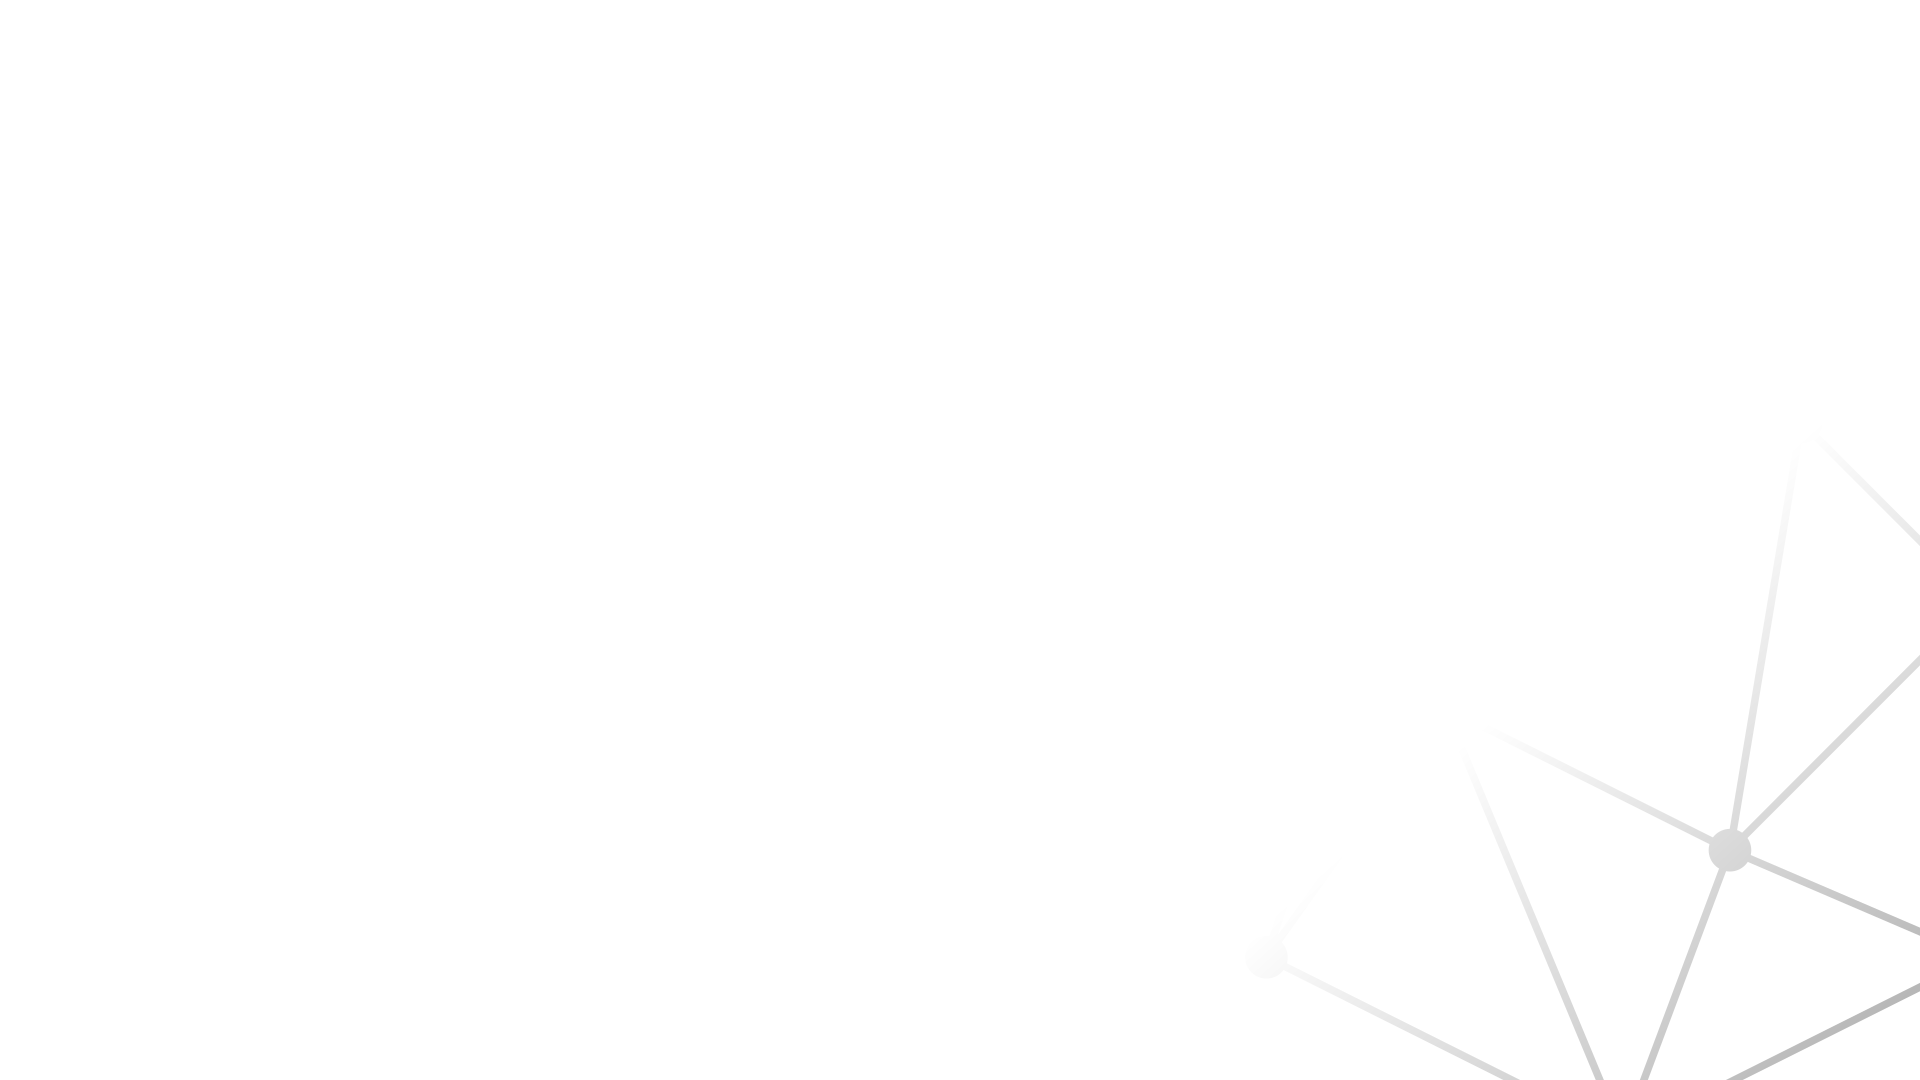
\includegraphics[width=\paperwidth,height=\paperheight]{images/background.png}
}

\setbeamertemplate{footline}[frame number]
\setbeamertemplate{navigation symbols}{}

\title{%
  Algorithmical Geometry: \\ Computation of Delaunay Triangulations \\ Using a Divide-and-Conquer Algorithm%
}
% \subtitle{Master's Thesis Defense and Presentation}
\author{Markus Pawellek}

\bibliography{references}

\begin{document}

\selectlanguage{english}

{ % all template changes are local to this group.
  \setbeamertemplate{navigation symbols}{}
  \begin{frame}<article:0>[plain]
    \begin{tikzpicture}[remember picture,overlay]
      \node[at=(current page.center)] {
        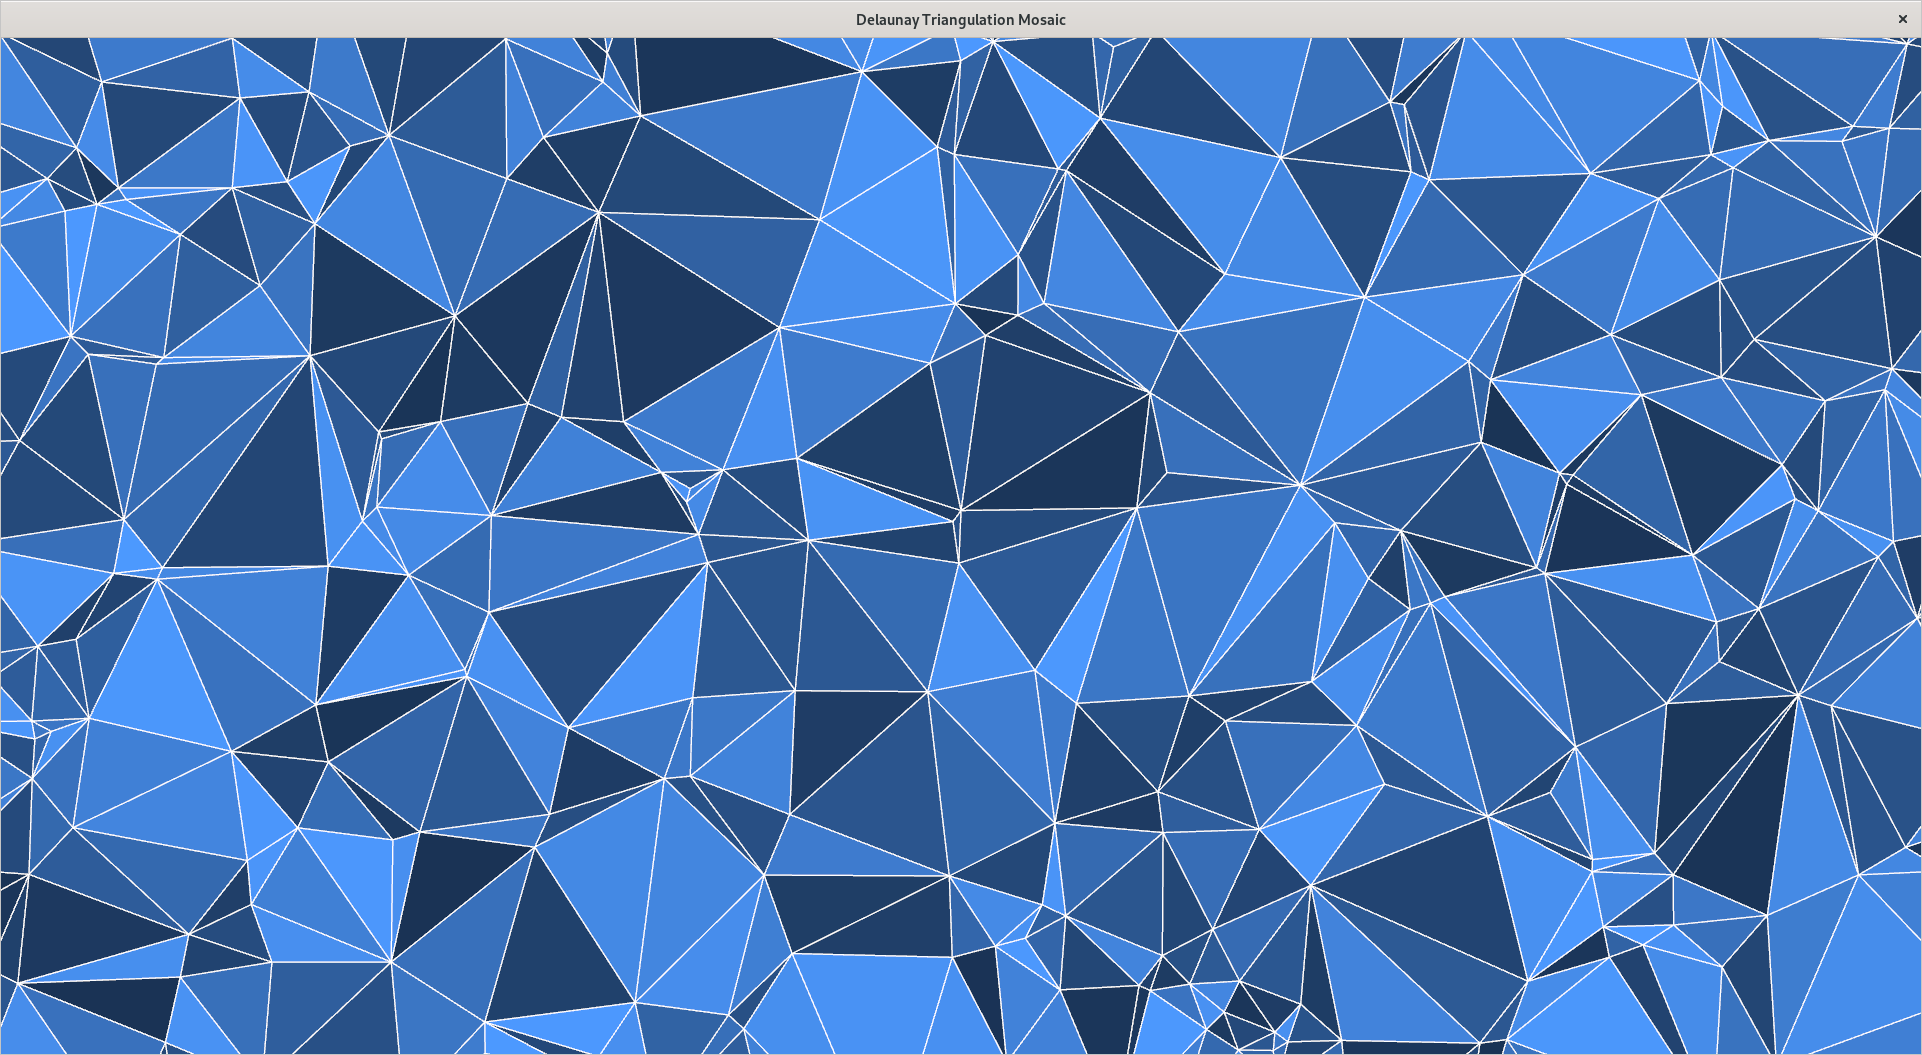
\includegraphics[keepaspectratio,
                         width=1.2\paperwidth,
                         height=\paperheight]{images/banner.png}
      };
    \end{tikzpicture}
  \end{frame}
}

\frame{\titlepage}
\begin{frame}{Outline}
  \footnotesize
  \hfill\parbox[t][7cm][l]{0.9\textwidth}{\tableofcontents}
\end{frame}

\section{Related Work}
  \begin{frame}{Related Work}
    % !!!Here should be an image of a wireframe for a mesh or a 3D grid for FEM simulation.
    % \bigskip
    \begin{minipage}[c]{0.49\textwidth}
      \begin{figure}
        \centering
        \includesvg[width=0.9\textwidth]{images/mesh-generation.svg}
      \end{figure}
      {%
        \fontsize{4}{5}\selectfont%
        *\url{https://upload.wikimedia.org/wikipedia/commons/b/b8/Approx-3tori.svg}, December 29, 2021%
      }
    \end{minipage}
    \hfill
    \begin{minipage}[c]{0.45\textwidth}
      \pause
      Educational Problems:
      \begin{itemize}
        \pause
        \item Many Resources
        \pause
        \item Duality to Voronoi Diagrams
        \pause
        \item%
          Multiple Algorithm Types: \\
          Incremental, Sweepline, Divide-and-Conquer
        \pause
        \item Varying Data Structures
      \end{itemize}
    \end{minipage}
  \end{frame}

  \begin{frame}{Related Work: References}
    \small
    \onslide<+->
    \begin{description}
      % This custom command does not work...
      % \newcommand\mycommand[1]{\item[\autocite{#1}] \citeauthor{#1}, \citetitle{#1}, \citeyear{#1}}
      \item<+->[\citeyear{lee1980}] \citeauthor{lee1980}, \citetitle{lee1980}
      \item<+->[\citeyear{guibas1985}] \textbf<7>{\citeauthor{guibas1985}, \citetitle{guibas1985}}
      \item<+->[\citeyear{dwyer1987}] \citeauthor{dwyer1987}, \citetitle{dwyer1987}
      \item<+->[\citeyear{shewchuk1996}] \citeauthor{shewchuk1996}, \citetitle{shewchuk1996}
      \item<+->[\citeyear{fuetterling2014}] \citeauthor{fuetterling2014}, \citetitle{fuetterling2014}
    \end{description}
  \end{frame}

\section{Mathematical Preliminaries}
  \begin{frame}{Mathematical Preliminaries: Triangle and Circumcircle}
    % Definition of a triangle can be difficult.
    % Hence, we use and indirect approach.
    % \onslide<+->
    \begin{minipage}[c]{0.45\textwidth}
      \textbf{Triangle} \\
      $A, B, C \in \setReal^2$ affinely independent \\
      define vertices of a triangle.

      \bigskip

      \pause
      \textbf{Circumcircle}\\
      Circle that intersects with \\
      all vertices of the triangle.
    \end{minipage}
    \hfill
    \begin{minipage}[c]{0.49\textwidth}
      \centering
      \onslide<1->
      \only<1>{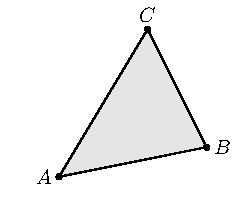
\includegraphics[width=0.9\textwidth]{figures/triangle.pdf}}%
      \only<2>{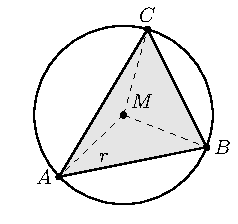
\includegraphics[width=0.9\textwidth]{figures/triangle-circumcirle.pdf}}
    \end{minipage}
  \end{frame}

  \begin{frame}{Mathematical Preliminaries: %
    \only<1>{Point Set}%
    \only<2>{Triangulation}%
    \only<3-5>{Delaunay Triangulation}%
  }
    \begin{minipage}[c]{0.45\textwidth}
      \onslide<+->
      \textbf{Point Set}\\
      $\mathscr{V}\subset\setReal^2$ finite, $\#\mathscr{V}\geq 3$, \\
      affinely span $\setReal^2$

      \bigskip

      \onslide<+->
      \textbf{Triangulation}\\
      Planar straight-line graph over $\mathscr{V}$ \\
      such that its edges form a maximal subset of non-crossing edges.

      \bigskip

      \onslide<+->
      \textbf{Delaunay Triangulation}\\
      Circumcircle of any triangle \\
      contains no other points of $\mathscr{V}$.
    \end{minipage}
    \hfill
    \begin{minipage}[c]{0.49\textwidth}
      \centering
      \onslide<1->
      \only<1>{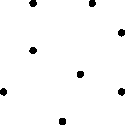
\includegraphics[width=\textwidth]{figures/point-set.pdf}}%
      \only<2>{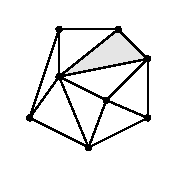
\includegraphics[width=\textwidth]{figures/triangulation.pdf}}%
      \only<3>{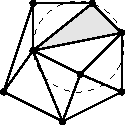
\includegraphics[width=\textwidth]{figures/triangulation-circumcircle.pdf}}%
      \only<4>{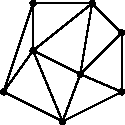
\includegraphics[width=\textwidth]{figures/delaunay-triangulation.pdf}}%
      \only<5>{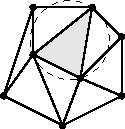
\includegraphics[width=\textwidth]{figures/delaunay-triangulation-circumcircle.pdf}}%
    \end{minipage}
  \end{frame}

  \begin{frame}{Mathematical Preliminaries: Properties}
    \begin{minipage}[c]{0.49\textwidth}
      \center
      \only<1-4>{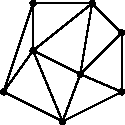
\includegraphics[width=\textwidth]{figures/delaunay-triangulation.pdf}}%
      \only<5>{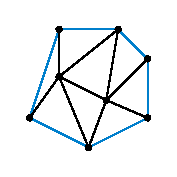
\includegraphics[width=\textwidth]{figures/delaunay-triangulation-convex-hull.pdf}}%
      \only<6>{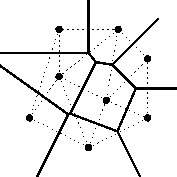
\includegraphics[width=\textwidth]{figures/delaunay-triangulation-voronoi.pdf}}%
    \end{minipage}
    \hfill
    \begin{minipage}[c]{0.49\textwidth}
      \begin{itemize}
        \item<2-> Existence is guaranteed
        \item<3-> Unique if there are no four points that are cocircular
        \item<4-> Optimality: maximization of the minimum angle of all angles
        \item<5-> Convex hull is contained
        \item<6-> Dual of Voronoi diagram
      \end{itemize}
    \end{minipage}
  \end{frame}

\section{Geometric Primitives}
  \begin{frame}{Geometric Primitives: Triangle Orientation}
    \begin{minipage}[c]{0.4\textwidth}
      %\begin{figure}
        \centering
        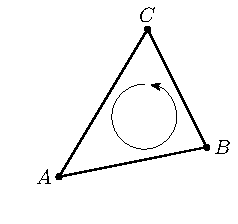
\includegraphics{figures/triangle-counterclockwise.pdf}
      %\end{figure}
    \end{minipage}
    \hfill
    $\longleftrightarrow$
    \hfill
    \begin{minipage}[c]{0.4\textwidth}
      %\begin{figure}
        \centering
        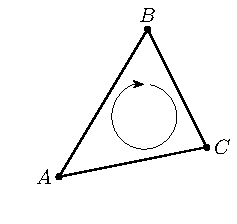
\includegraphics{figures/triangle-clockwise.pdf}
      %\end{figure}
    \end{minipage}

    \pause
    Counterclockwise Orientation
    $\quad\iff\quad$ $C$ is left of $\overline{AB}$

    \bigskip

    \pause
    \begin{mybox}
    \[
      0 <
      \begin{vmatrix}
        A_x & A_y & 1 \\
        B_x & B_y & 1 \\
        C_x & C_y & 1 \\
      \end{vmatrix}
      \pause
      =
      \begin{vmatrix}
        B_x - A_x & B_y - A_y \\
        C_x - A_x & C_y - A_y \\
      \end{vmatrix}
      \pause
      =
      \det
      \begin{pmatrix}
        B-A && C-A
      \end{pmatrix}
    \]
    \end{mybox}
  \end{frame}

  \begin{frame}{Geometric Primitives: Inside Circumcircle}
    \pause
    \begin{minipage}[c]{0.49\textwidth}
      \begin{mybox}
        \[
          0 <
          \begin{vmatrix}
            A_x & A_y & A_x^2 + A_y^2 & 1 \\
            B_x & B_y & B_x^2 + B_y^2 & 1 \\
            C_x & C_y & C_x^2 + C_y^2 & 1 \\
            D_x & D_y & D_x^2 + D_y^2 & 1 \\
          \end{vmatrix}
        \]
        \pause
        \[
          =
          \begin{aligned}[t]
            &\scalarProduct{x}{\mathrm{adj}\begin{pmatrix}u & v \end{pmatrix}^\mathrm{T} \begin{pmatrix}\norm{u}^2 \\ \norm{v}^2 \end{pmatrix}} \\
            &- \det\begin{pmatrix}u & v \end{pmatrix}\norm{x}^2
          \end{aligned}
        \]
      \end{mybox}
      $u \define B-A ,\quad v \define C-A ,\quad x \define D-A$
    \end{minipage}
    \hfill
    \begin{minipage}[c]{0.49\textwidth}
      \center
      \onslide<1->
      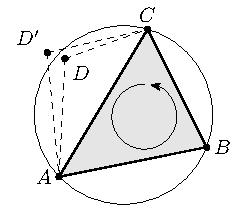
\includegraphics[width=0.9\textwidth]{figures/inside-circumcircle.pdf}
    \end{minipage}
  \end{frame}

\section{Quad-Edge Data Structure}
  \begin{frame}{Quad-Edge Data Structure: Scheme}
    \begin{minipage}[c]{0.49\textwidth}
      Edge-Based List-Like Data Structure \\
      for Storing Neighbor Information:
      \onslide<+->
      \begin{itemize}
        \item<+-> Directed edges for vertices
        \item<+-> Pointer to ccw. next directed edge with same origin vertex
        \item<+-> Directed dual edges for adjacent faces
        \item<+-> Pointer to ccw. next directed dual edge with same origin face
      \end{itemize}
    \end{minipage}
    \hfill
    \begin{minipage}[c]{0.49\textwidth}
      \center
      \only<1>{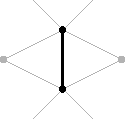
\includegraphics[width=0.9\textwidth]{figures/quad-edge-empty.pdf}}%
      \only<2-3>{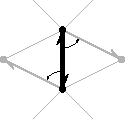
\includegraphics[width=0.9\textwidth]{figures/quad-edge.pdf}}%
      \only<4-5>{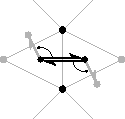
\includegraphics[width=0.9\textwidth]{figures/quad-edge-dual.pdf}}%
      \only<6->{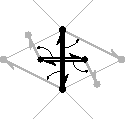
\includegraphics[width=0.9\textwidth]{figures/quad-edge-both.pdf}}%
    \end{minipage}
  \end{frame}

  \begin{frame}{Quad-Edge Data Structure: Implementation}
    \begin{minipage}[c]{0.49\textwidth}
      %\onslide<1>
      \only<1>{%
        \begin{figure}
          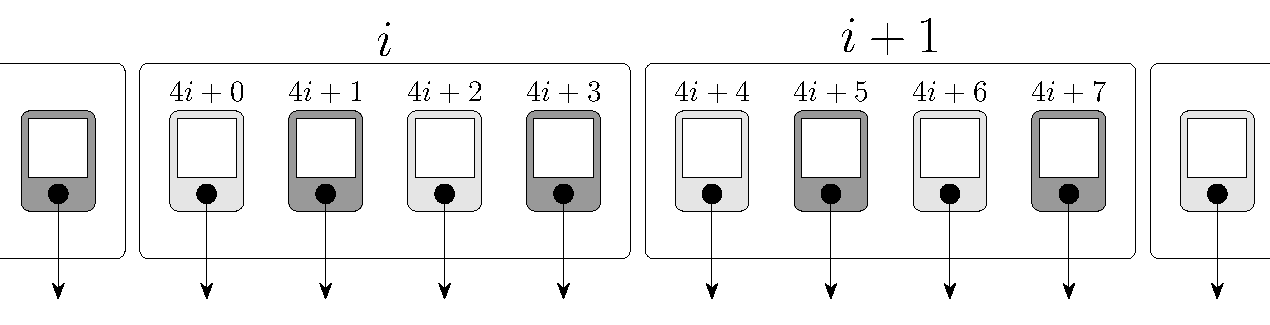
\includegraphics[width=\textwidth]{figures/quad-edge-struct.pdf}
        \end{figure}%
        \begin{mybox}
          \center
          \vspace{-1em}
          \inputCodeBlock{listings/quad-edge-algebra.cpp}
        \end{mybox}%
      }%
      %\onslide<2>
      \only<2>{%
        %\begin{mybox}
        %  \inputCodeBlock{listings/quad-edge-algebra-operations.cpp}
        %\end{mybox}}%
        \begin{figure}
          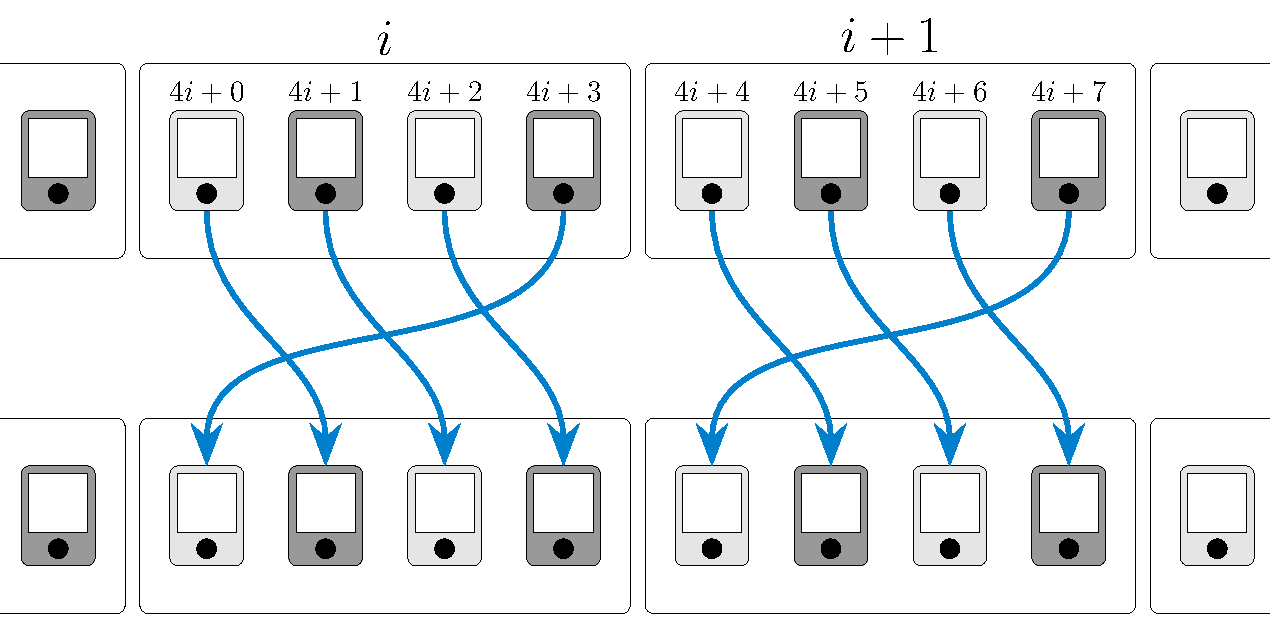
\includegraphics[width=\textwidth]{figures/quad-edge-struct-rot.pdf}
        \end{figure}%
        \begin{mybox}
          \[
            \function{\mathrm{rot}}{\setNatural_0}{\setNatural_0}
          \]
          \[
            \mathrm{rot}(x) = 4 \cdot \floorBrackets{\frac{x}{4}} + (x+1 \mod 4)
          \]
        \end{mybox}%
      }%
    \end{minipage}
    \hfill
    \begin{minipage}[c]{0.49\textwidth}
      \center
      \only<1>{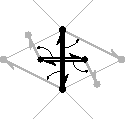
\includegraphics[width=0.9\textwidth]{figures/quad-edge-both.pdf}}%
      \only<2>{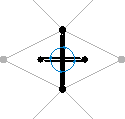
\includegraphics[width=0.9\textwidth]{figures/quad-edge-rot.pdf}}%
    \end{minipage}
  \end{frame}

  \begin{frame}{Quad-Edge Data Structure: Edge Functions and Operators}
    \begin{figure}
      \center
      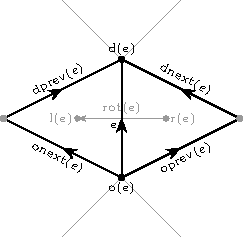
\includegraphics[height=0.6\textheight]{figures/quad-edge-vertex-functions.pdf}
      \hspace{2em}
      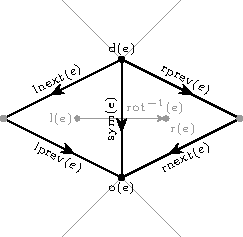
\includegraphics[height=0.6\textheight]{figures/quad-edge-face-functions.pdf}
    \end{figure}
    \onslide<+->
    \begin{itemize}
      \item<+-> Create a new edge
      \item<+-> Delete existing edge
      \item<+-> Connect points by a new edge
    \end{itemize}
  \end{frame}

\section{Algorithm}
  \begin{frame}{Algorithm: Overview}
    %\only<1>{%
      \onslide<+->
      \onslide<+->
      \begin{mybox}
        \textbf{Triangulation Algorithm}
        \begin{enumerate}
          \item<+-> Sort the given point set by increasing $x$ coordinate.
          \item<+-> Triangulate sorted point set.
        \end{enumerate}
      \end{mybox}%
      \bigskip
      %\begin{itemize}
      %  \item Preprocessing Step with Complexity $\mathscr{O}(n\log n)$
      %  \item Sorting of points makes split constant time operation
      %\end{itemize}%
    %}%
    %\only<2>{%
    \bigskip
      \onslide<+->
      \begin{mybox}
        \textbf{Subroutine: Triangulate}
        \begin{enumerate}
          \item<+-> If point count is smaller than four, make edge or triangle and return.
          %\item If $\#\mathscr{V}<4$ then make $\mathscr{T}(\mathscr{V})$ an edge or a triangle and break
          %\item $\mathbf{if}\ \#\mathscr{V}<4 \ \mathbf{then}$ \\ $\quad \mathscr{T}(\mathscr{V}) \longleftarrow \mathrm{edge\_or\_triangle}(\mathscr{V})$ \\ $\quad \mathbf{return}$
            %\begin{enumerate}
            %  \item $\mathscr{T}(\mathscr{V}) \longleftarrow \mathrm{edge or triangle}(\mathscr{V})$
            %  \item $\mathrm{break}$
            %\end{enumerate}
          %\item Separate $\mathscr{V}$ into halves $\mathscr{L}$ and $\mathscr{R}$
          \item<+-> Split point set into left and right half.
          \item<+-> Triangulate left and right half.
          \item<+-> Merge left and right triangulations.
          %\item $(\mathscr{L},\mathscr{R}) \longleftarrow \mathrm{split}(\mathscr{V})$
          %\item Triangulate $\mathscr{L}$ and $\mathscr{R}$ into $\mathscr{T}(\mathscr{L})$ and $\mathscr{T}(\mathscr{R})$
          %\item $(\mathscr{T}(\mathscr{L}), \mathscr{T}(\mathscr{R})) \longleftarrow (\mathrm{triangulate}(\mathscr{L}),\mathrm{triangulate}(\mathscr{R}))$
          %\item $\mathscr{T}(\mathscr{L}) \longleftarrow \mathrm{triangulate}(\mathscr{L})$
          %\item $\mathscr{T}(\mathscr{R}) \longleftarrow \mathrm{triangulate}(\mathscr{R})$
          %\item Merge $\mathscr{T}(\mathscr{L})$ and $\mathscr{T}(\mathscr{R})$
          %\item $\mathscr{T}(\mathscr{V}) \longleftarrow \mathrm{merge}(\mathscr{T}(\mathscr{L}), \mathscr{T}(\mathscr{R}))$
        \end{enumerate}
      \end{mybox}%
      %\begin{itemize}
      %  \item Divide-and-Conquer Algorithm
      %  \item Key is merge step
      %\end{itemize}%
    %}%
  \end{frame}

  \begin{frame}{Algorithm: Merge Triangulations Example}
    \only<+>{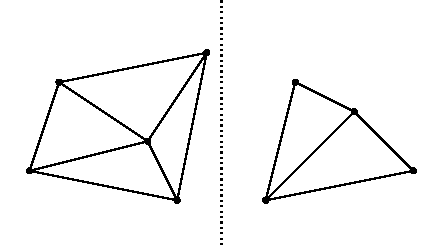
\includegraphics[width=\textwidth]{figures/merge-empty.pdf}}%
    \only<+>{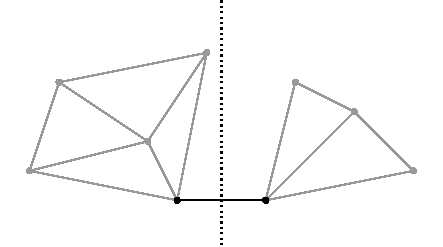
\includegraphics[width=\textwidth]{figures/merge-lct.pdf}}%
    \only<+>{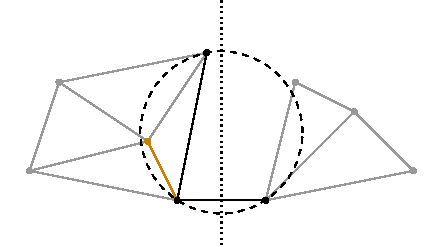
\includegraphics[width=\textwidth]{figures/merge-invalid-edge-circle-test.pdf}}%
    \only<+>{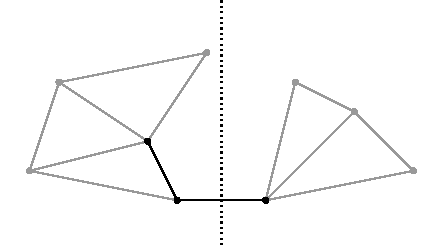
\includegraphics[width=\textwidth]{figures/merge-invalid-edge-removal.pdf}}%
    \only<+>{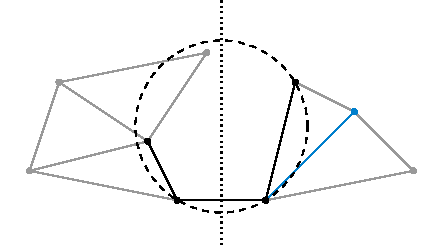
\includegraphics[width=\textwidth]{figures/merge-invalid-edge-circle-test-right.pdf}}%
    \only<+>{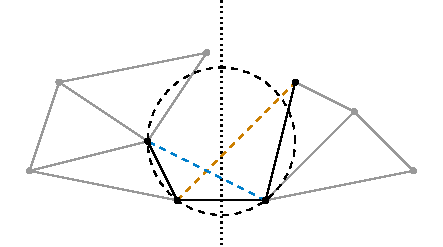
\includegraphics[width=\textwidth]{figures/merge-cross-edge-circle-test.pdf}}%
    \only<+>{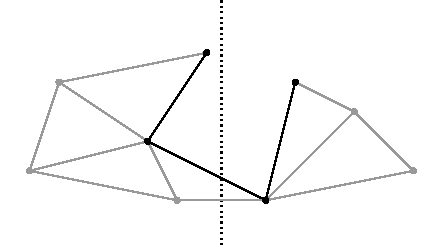
\includegraphics[width=\textwidth]{figures/merge-cross-edge-insertion.pdf}}%
    \only<+>{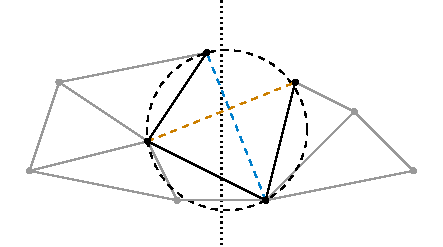
\includegraphics[width=\textwidth]{figures/merge-second-circle-test.pdf}}%
    \only<+>{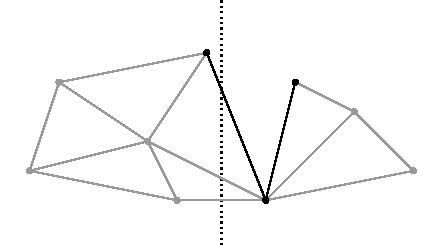
\includegraphics[width=\textwidth]{figures/merge-second-cross-edge.pdf}}%
    \only<+>{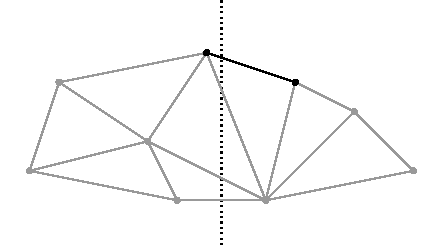
\includegraphics[width=\textwidth]{figures/merge-uct.pdf}}%
    \only<+>{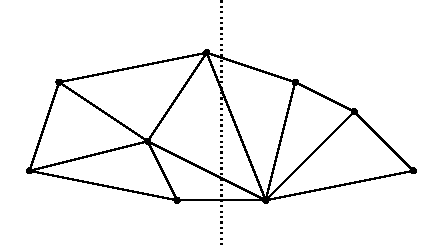
\includegraphics[width=\textwidth]{figures/merge-finish.pdf}}%
  \end{frame}

  \begin{frame}{Algorithm: Merge Triangulations}
    \onslide<+->
    \onslide<+->
    \begin{mybox}
      \textbf{Subroutine: Merge Triangulations}
      \begin{enumerate}
        %\item $\mathscr{T}(\mathscr{V}) \longleftarrow \mathscr{T}(\mathscr{L}) \cup \mathscr{T}(\mathscr{R})$
        \item<+-> Compute and add lower common tangent.
        %\item Find lower common tangent of $\mathscr{L}$ and $\mathscr{R}$
        %\item $b \longleftarrow \mathrm{lower\_common\_tangent}(\mathscr{L}, \mathscr{R})$
        %\item Add lower common tangent as $b$
        %\item $\mathscr{T}(\mathscr{V}) \longleftarrow \mathscr{T}(\mathscr{V}) \cup b$
        %\item Loop until $b$ is upper common tangent:
        \item<+-> Use lower common tangent as baseline.
        \item<+-> Loop until baseline becomes upper common tangent:
          \begin{enumerate}
            \item<+-> Remove invalid edges adjacent to and above baseline.
            \item<+-> Insert cross edge above baseline.
            \item<+-> Make this cross edge the new baseline.
          \end{enumerate}
        %\item $\mathbf{while} \ b \neq \mathrm{upper\_common\_tangent}(\mathscr{L}, \mathscr{R})$
        %  \begin{enumerate}
        %    \item $\mathscr{T}(\mathscr{V}) \longleftarrow \mathscr{T}(\mathscr{V}) \setminus \mathrm{invalid\_edges}(\mathscr{T}(\mathscr{L}), b)$
        %    \item $\mathscr{T}(\mathscr{V}) \longleftarrow \mathscr{T}(\mathscr{V}) \setminus \mathrm{invalid\_edges}(\mathscr{T}(\mathscr{R}), b)$
        %    %\item Insert cross edge $c$ above $b$
        %    \item $b \longleftarrow \mathrm{cross\_edge}(\mathscr{T}(\mathscr{V}), b)$
        %    \item $\mathscr{T}(\mathscr{V}) \longleftarrow \mathscr{T}(\mathscr{V}) \cup b$
        %  \end{enumerate}
      \end{enumerate}
    \end{mybox}
    \begin{itemize}
      \item linear complexity by using Euler's formula for planar graphs
      \item computation of lower common tangent
      \item circle test for adjacent edges
      \item circle test for cross edge
    \end{itemize}
  \end{frame}

  %\begin{frame}{Algorithm: Insert Cross Edges}
  %  \begin{mybox}
  %    \textbf{Subroutine: Remove Invalid Edge}
  %    \begin{enumerate}
  %      \item While adjacent edge lies in circumcircle
  %      \item remove edge
  %    \end{enumerate}
  %  \end{mybox}%
  %  \begin{mybox}
  %    \textbf{Subroutine: Insert Cross Edge}
  %    \begin{enumerate}
  %      \item Insert cross edge by using circle test
  %    \end{enumerate}
  %  \end{mybox}%
  %\end{frame}

  %\begin{frame}{Algorithm: Lower Common Tangent}
  %  \begin{mybox}
  %    \textbf{Subroutine: Lower Common Tangent}
  %    \begin{enumerate}
  %      \item $l$ and $r$ as inner convex hull edges
  %      \item Loop:
  %      \begin{enumerate}
  %        \item If $\mathrm{leftof}(\mathrm{o}(r), l)$ then $l \longleftarrow \mathrm{lnext}(l)$
  %        \item If $\mathrm{rightof}(\mathrm{o}(l), r)$ then $r \longleftarrow \mathrm{rprev}(r)$
  %        \item Else break
  %      \end{enumerate}
  %    \end{enumerate}
  %  \end{mybox}
  %\end{frame}

  \begin{frame}{Algorithm: Complexity}
    \begin{minipage}[c]{0.49\textwidth}
      \begin{itemize}
        \item Use master theorem
        \item Merge step is linear in point count
      \end{itemize}
      \[
        t(n) = 2 t\roundBrackets{\frac{n}{2}} + \mathscr{O}(n)
      \]
      \[
        \mathscr{O}(n\log n)
      \]
    \end{minipage}
    \hfill
    \begin{minipage}[c]{0.49\textwidth}
      \begin{mybox}
        \textbf{Subroutine: Triangulate}
        \begin{enumerate}
          \item If point count is smaller than four, make edge or triangle and return.
          \item Split point set into left and right half.
          \item Triangulate left and right half.
          \item Merge left and right triangulations.
        \end{enumerate}
      \end{mybox}%
    \end{minipage}
  \end{frame}

  \begin{frame}{Algorithm: Correctness}
    Proof by induction: \\
    Show that for two given Delaunay triangulations $\mathscr{T}(\mathscr{L})$ and $\mathscr{T}(\mathscr{R})$ separated by a vertical line the merge subroutine generates a Delaunay triangulation $\mathscr{T}(\mathscr{L}\cup\mathscr{R})$.
    \begin{itemize}
      \item For two Delaunay triangulations separated by a vertical line, it is enough to remove inner edges and insert cross edges.
      \item Common tangents are elements of the Delaunay triangulation.
      \item Removed edges are indeed not Delaunay.
      \item Insertion of cross edges generates new Delaunay triangle.
      \item There are no other edges that have to be removed.
      \item Theorem: Algorithm is correct.
    \end{itemize}
  \end{frame}

\section{Implementation Notes}
  \begin{frame}{Implementation Notes}
    \begin{itemize}
      \item Geometric Primitives need exact computation and therefore arbitrary precision
      \item still no robust split, use Dwyer instead (no sorting, parallelization)
      \item triangular data structure increases speed but algorithm is more complicated
      \item Divide-and-conquer variant seems to be most powerful and robust
    \end{itemize}
  \end{frame}

\section{Applications}

\section{Conclusions}
  \begin{frame}{Conclusions}
    \textbf{Summary:}
    \begin{itemize}
      \item Delaunay triangulation can be generated by given divide-and-conquer algorithm in $\mathscr{O}(n\log n)$
      \item Data structure needs to store neighbor information
    \end{itemize}
    \bigskip
    \textbf{Future Work:}
    \begin{itemize}
      \item Use triangular data structure instead of quad-edge data structure
      \item Use \citeauthor{dwyer1987}'s approach to make algorithm more robust
      \item Parallelization
    \end{itemize}
  \end{frame}


\setcounter{backupcounter}{\value{framenumber}}

\begin{frame}[plain]
  \vfill
  \centering
  \begin{beamercolorbox}[sep=8pt,center,shadow=true,rounded=true]{title}
    \usebeamerfont{title}%
    Thank you for Your Attention!%
    \par%
  \end{beamercolorbox}
  \vfill
\end{frame}

\begin{frame}[plain]
  \frametitle{References}
  % \tiny
  \AtNextBibliography{\tiny}
  \begin{multicols}{2}
    \nocite{*}
    \printbibliography
  \end{multicols}
\end{frame}

\setcounter{framenumber}{\value{backupcounter}}

\end{document}
